\chapter{Implementation}\label{ch:implementation}

After the wait-free algorithms were identified and analysed, the next sub-goal to find the best wait-free algorithms is to implement them like already said in \cref{sec:objective}. The algorithms were implemented and published in the accompanying GitHub repository in \cite{githubMA}, where complete implementation of the algorithms can be found. This chapter will present the implementation details of the concurrent queue algorithms seen in \cref{ch:choosing-the-optimal-wait-free-data-structure} in Rust, focusing on the adaptations necessary for \ac{IPC} over shared memory. While the algorithmic logic of each queue has already been discussed in \cref{ch:choosing-the-optimal-wait-free-data-structure}, the implementation required slight deviations to support \ac{IPC} over shared memory. This includes ensuring correct cache alignment, correctly implementing various atomic primitives, and correctly implementing the logic for shared memory support using short example snippets of the actual Rust implementation from the GitHub repository or some general examples. This does not include showing again the same algorithmic logic, just in an actual programming language instead of pseudocode, since that would be redundant. This chapter will give the necessary details to understand how to implement the algorithms in Rust and how to adapt them for \ac{IPC} over shared memory.

\section{Shared Memory Management for \acf{IPC}}

\ac{IPC} through shared memory requires slightly different approaches compared to multi-threaded heap-based communication. The primary constraint is that shared memory regions may be mapped at different virtual addresses in different processes, requiring all data structures to be completely position-independent. Additionally, dynamic memory allocation is not possible within shared memory regions, necessitating buffer allocation from a pre-allocated memory pool for all dynamic data structures. Threads, on the other hand, can use the process-private heap for dynamic memory allocation, whose memory layout is shared between threads on the same process, but not between processes.  

\subsection{Shared Memory Size Calculation}

Each queue provides a method to calculate the exact shared memory size required. This calculation determines how much memory to allocate from the operating system. The following examples from BQueue and \ac{wCQ} demonstrate both simple and complex size calculations as needed:

\begin{lstlisting}[language=Rust, style=boxed, caption={Shared memory size calculation methods}, label={lst:size-calculation}]
// From BQueue - simple calculation
pub const fn shared_size(capacity: usize) -> usize {
    mem::size_of::<Self>()                              // Queue structure
        + capacity * mem::size_of::<MaybeUninit<T>>()   // Data storage
        + capacity * mem::size_of::<AtomicBool>()       // Validity flags
}

// From WCQueue - complex layout calculation
fn layout(num_threads: usize, num_indices: usize) -> (Layout, [usize; 4]) {
    let ring_size = num_indices.next_power_of_two();
    let capacity = ring_size * 2;
    
    let root = Layout::new::<Self>();
    let (l_aq_entries, o_aq_entries) = root
        .extend(Layout::array::<EntryPair>(capacity).unwrap())
        .unwrap();
    let (l_fq_entries, o_fq_entries) = l_aq_entries
        .extend(Layout::array::<EntryPair>(capacity).unwrap())
        .unwrap();
    let (l_records, o_records) = l_fq_entries
        .extend(Layout::array::<ThreadRecord>(num_threads).unwrap())
        .unwrap();
    let (l_final, o_data) = l_records
        .extend(Layout::array::<DataEntry<T>>(num_indices).unwrap())
        .unwrap();
    
    (l_final.pad_to_align(), [o_aq_entries, o_fq_entries, o_records, o_data])
}

pub fn shared_size(num_threads: usize) -> usize {
    let (_layout, _offsets) = Self::layout(num_threads, num_indices);
    _layout.size()  // Total bytes needed for mmap
}
\end{lstlisting}

The size calculation accounts for all components, including alignment padding. Some queues like \ac{wCQ} use Rust's \texttt{Layout} API shown in lines 9 to 26 to ensure proper alignment and correctly calculated offsets. For simple queues like BQueue, manual calculation like in lines 2 to 6 suffices.

\subsection{Shared Memory Allocation}

Once the required size is calculated, the following functions in \cref{lst:map-shared} used in all benchmarks demonstrate how to allocate and deallocate the required shared memory regions using \texttt{mmap}:

\begin{lstlisting}[language=Rust, style=boxed, caption={Shared memory allocation using mmap}, label={lst:map-shared}]
unsafe fn map_shared(bytes: usize) -> *mut u8 {
    let ptr = libc::mmap(
        ptr::null_mut(),
        bytes,                                    // Size from shared_size()
        libc::PROT_READ | libc::PROT_WRITE,
        libc::MAP_SHARED | libc::MAP_ANONYMOUS,   // Shared between processes
        -1,
        0,
    );
    if ptr == libc::MAP_FAILED {
        panic!("mmap failed: {}", std::io::Error::last_os_error());
    }
    ptr.cast()
}

// Cleanup function
unsafe fn unmap_shared(ptr: *mut u8, len: usize) {
    if libc::munmap(ptr.cast(), len) == -1 {
        panic!("munmap failed: {}", std::io::Error::last_os_error());
    }
}
\end{lstlisting}

The \texttt{MAP\_SHARED} flag ensures that modifications to the memory region are visible to all processes that map it. The \texttt{MAP\_ANONYMOUS} flag creates memory not backed by a file. The \texttt{bytes} parameter on line 4 comes directly from the \texttt{shared\_size()} calculation earlier.

\subsection{Memory Layout and Initialisation}

After allocating the shared memory region, the components needed by the queue implementations need to be initialised. All queue implementations follow a consistent pattern for shared memory initialisation. The initialisation function receives the pre-allocated memory pointer and organises components within that memory region. The most complex example, the WCQueue from \cref{subsubsec:wcq}, demonstrates how multiple components are laid out in shared memory with proper alignment:

\begin{lstlisting}[language=Rust, style=boxed, caption={Memory layout initialisation in WCQueue}, label={lst:wcqueue-init}]
pub unsafe fn init_in_shared(mem: *mut u8, num_threads: usize) -> &'static mut Self {
    let mut current_offset = 0usize;
    
    // Align and place queue structure
    current_offset = (current_offset + self_align - 1) & !(self_align - 1);
    let q_ptr = mem.add(current_offset) as *mut Self;
    current_offset += mem::size_of::<Self>();
    
    // Align and place entry arrays
    current_offset = (current_offset + entry_align - 1) & !(entry_align - 1);
    let aq_entries = mem.add(current_offset) as *mut EntryPair;
    current_offset += capacity * mem::size_of::<EntryPair>();
    
    // Initialise structures in-place
    ptr::write(q_ptr, Self {
        aq_entries_offset: current_offset,
        base_ptr: mem,  // Store base pointer for offset calculations
        // Store offsets instead of pointers
    });
    
    &mut *q_ptr
}
\end{lstlisting}

The alignment calculation in line 5 ensures that each component starts at a properly aligned address. This is crucial for atomic operations, which often require natural alignment. The queue structure stores offsets relative to the base pointer rather than absolute pointers in line 16, ensuring position independence. When accessing these components later, the offset is added to the base pointer, as demonstrated in \cref{lst:position-independent}.

\begin{lstlisting}[language=Rust, style=boxed, caption={Position-independent component access}, label={lst:position-independent}]
unsafe fn get_entry(&self, entries_offset: usize, idx: usize) -> &EntryPair {
    let entries = self.base_ptr.add(entries_offset) as *const EntryPair;
    &*entries.add(idx)
}
\end{lstlisting}

\subsection{Node Allocation from Pre-allocated Memory Pools}

Some queues as seen in \cref{ch:choosing-the-optimal-wait-free-data-structure} use dynamic memory allocation within the process-private heap. For the \ac{IPC} over shared memory use case of this thesis that is not possible, because in shared memory dynamic memory allocations or deallocations with \texttt{malloc} or \texttt{free} are not possible, since that allocates from process-private heaps that are not available for other processes. Therefore, all queues that would normally allocate memory dynamically have been adapted to allocate from the initialised pre-allocated memory pool. As an example, the Jiffy Queue algorithm from \cref{subsubsec:jiffy-mpsc-queue} shows a dynamic heap allocation method to allocate new buffers to insert them into the linked list. This was adapted to \ac{IPC} over shared memory in Rust by a pool allocation system with free lists that is similarly implemented for all other queues needing dynamic memory allocation, as shown in \cref{lst:pool-allocation}.

\begin{lstlisting}[language=Rust, style=boxed, caption={Lock-free memory pool allocation}, label={lst:pool-allocation}]
unsafe fn alloc_node_array_slice(&self) -> *mut Node<T> {
    // Try reuse from free list first
    loop {
        let free_head = self.node_array_slice_free_list_head.load(Ordering::Acquire);
        if free_head.is_null() {
            break;
        }
        
        let next_free = (*(free_head as *mut AtomicPtr<Node<T>>))
            .load(Ordering::Acquire);
            
        if self.node_array_slice_free_list_head.compare_exchange(
            free_head, 
            next_free, 
            Ordering::AcqRel, 
            Ordering::Acquire
        ).is_ok() {
            return free_head;
        }
    }
    
    // Allocate from pre-allocated pool
    let nodes_needed = self.buffer_capacity_per_array;
    let start_idx = self.node_arrays_next_free_node_idx
        .fetch_add(nodes_needed, Ordering::AcqRel);
        
    if start_idx + nodes_needed > self.node_arrays_pool_total_nodes {
        self.node_arrays_next_free_node_idx
            .fetch_sub(nodes_needed, Ordering::Relaxed);
        return ptr::null_mut(); // Pool exhausted
    }
    
    self.node_arrays_pool_start.add(start_idx)
}
\end{lstlisting}

This implementation maintains a free list using \ac{CAS} operations in lines 12 to 16. When the free list is empty, it falls back to allocate from the pre-allocated pool seen in lines 23 and 24. The \texttt{fetch\_add} operation atomically increments the allocation index, ensuring process-safe allocation. If the pool is exhausted, the operation fails by returning a null pointer in line 30.

\section{Cache Line Optimisation}
Processors transfer data between cores in cache line units, explained in \cref{subsubsec:lamport-circular-buffer-queue}. When multiple processes access data on the same cache line, even if different variables, the cache coherence protocol causes the cache line to bounce between cores, degrading execution times.

\subsection{Explicit Cache Line Padding}

In \cref{ch:choosing-the-optimal-wait-free-data-structure}, multiple queues were shown that describe separating the cache line. To show how this is done in rust the \ac{BLQ} explained in \cref{subsec:single-producer-and-single-consumer} will be taken to show how to explicitly separate the cache lines, as shown in \cref{lst:cache-separation}.

\begin{lstlisting}[language=Rust, style=boxed, caption={Cache line separation in BlqQueue}, label={lst:cache-separation}]
const CACHE_LINE_SIZE: usize = 64;

#[repr(C)]
#[cfg_attr(any(target_arch = "x86_64", target_arch = "aarch64"), repr(align(64)))]
pub struct SharedIndices {
    pub write: AtomicUsize,  // Producer's cache line
    pub read: AtomicUsize,   // Consumer's cache line
}

#[repr(C, align(64))]
struct ProducerPrivate {
    read_shadow: usize,      // Local copy to avoid false sharing
    write_priv: usize,       // Producer-only write position
}

#[repr(C, align(64))]
struct ConsumerPrivate {
    write_shadow: usize,     // Local copy to avoid false sharing
    read_priv: usize,        // Consumer-only read position
}
\end{lstlisting}

The \texttt{\#[repr(C)]} attribute ensures C-compatible memory layout, while \newline \texttt{\#[repr(align(64))]} forces the structure to start at a cache line boundary, shown in lines 4 and 10. Although \texttt{SharedIndices} contains only two \texttt{usize} values with 16 bytes total, the alignment ensures they reside in separate cache lines. The producer updates \texttt{write} while the consumer updates \texttt{read}, preventing false sharing. The shadow copies \texttt{read\_shadow} in line 12 and \texttt{write\_shadow} in line 18 ensure that producer and consumer work on different cache lines, preventing the cache lines from bouncing between the producer process and consumer process.

Similarly, all queues that need this kind of cache line separation use this pattern to ensure that the producer and consumer do not share cache lines, preventing false sharing, leading to cache lines bouncing between cores.

\subsection{Manual Padding Arrays}

For structures where alignment alone is insufficient, manual padding arrays provide a solution, as demonstrated in \cref{lst:manual-padding}. This is used in all queues needing manual padding. As an example, the implementation of the David queue explained in \cref{subsubsec:david-queue} uses manual padding.

\begin{lstlisting}[language=Rust, style=boxed, caption={Manual padding for exact cache line control}, label={lst:manual-padding}]
#[repr(C, align(64))]
struct FetchIncrement {
    value: AtomicUsize,
    _padding: [u8; CACHE_LINE_SIZE - std::mem::size_of::<AtomicUsize>()],
}

#[repr(C, align(64))]
struct Node<T> {
    val: Option<T>,
    next: AtomicPtr<Node<T>>,
    _padding: [u8; CACHE_LINE_SIZE - 24], // Fill remaining cache line
}
\end{lstlisting}

The padding array size is calculated to fill the remainder of the cache line seen in lines 4 and 11. For \texttt{FetchIncrement}, the \texttt{AtomicUsize} occupies 8 bytes, so 56 bytes of padding complete the 64-byte cache line. This ensures each \texttt{FetchIncrement} instance occupies exactly one cache line, preventing false sharing in arrays of such structures, as required by the DavidQueue implementation from \cref{subsubsec:david-queue}.

\section{Atomic Primitives Implementation}

The algorithms in \cref{ch:choosing-the-optimal-wait-free-data-structure} all use different kinds of atomic primitives. To implement them, rust provides a set of atomic operations with explicit memory ordering semantics, allowing control over synchronisation order. This section shows how in general the atomic operations from \cref{ch:choosing-the-optimal-wait-free-data-structure} are implemented in Rust across all queues, explained with specific examples. In rust, atomic primitives can only be called on atomic types. Hence variables that are used in atomic operations must be defined as atomic types.

\subsection{\acf{FAA}}

The rust implementations of DQueue, BQueue and \ac{wCQ} explained in \cref{ch:choosing-the-optimal-wait-free-data-structure} are a good example to understand how to implement \ac{FAA} called \texttt{fetch\_add(v, ordering)} in rust.

\begin{lstlisting}[language=Rust, style=boxed, caption={Fetch-and-add with different memory orderings}, label={lst:fetch-and-add}]
// From Jiffy - Allocate multiple nodes at once
let start_node_idx = self
    .node_arrays_next_free_node_idx
    .fetch_add(nodes_needed, Ordering::AcqRel);

// From BQueue - private counter with relaxed ordering
let idx = self.next_item.fetch_add(1, Ordering::Relaxed);

// From WCQueue - with sequential consistency for wait-free algorithm
let seqid = self.tail.fetch_add(1, Ordering::SeqCst);
\end{lstlisting}

In Rust, \ac{FAA} is a method call on atomic types as seen in line 4. In \cref{lst:fetch-and-add}, the memory ordering parameter added as the second argument after the value to add determines the synchronisation order of \ac{FAA}. \texttt{Ordering::Relaxed} in line 7 provides no synchronisation, suitable for private counters. \texttt{Ordering::AcqRel} in line 4 ensures acquire semantics for the read and release semantics for the write, establishing happens-before relationships as required by the DQueue algorithm. \texttt{Ordering::SeqCst} in line 10 provides the strongest guarantees, ensuring a total order across all sequentially consistent operations, necessary for the complex \ac{wCQ}. One simple solution would be to always use \texttt{Ordering::SeqCst} for all operations, but that would reduce the execution times of the algorithms in a significant way. Consequently, it is important to analyse the algorithms from \cref{ch:choosing-the-optimal-wait-free-data-structure} to understand which memory ordering is needed for which operation.

\subsection{\acf{CAS}}

The implementation of \ac{wCQ} shows how to implement \ac{CAS}, called \newline \texttt{compare\_exchange(old\_value, new\_value, ordering\_on\_success, \newline ordering\_on\_failure)} in rust, as shown in \cref{lst:compare-and-swap}.

\begin{lstlisting}[language=Rust, style=boxed, caption={Compare-and-swap variants and usage patterns}, label={lst:compare-and-swap}]
// Strong CAS with sequential consistency (from wcqueue)
match entry.value.compare_exchange(
    packed,
    new_packed,
    Ordering::SeqCst,    // Success ordering
    Ordering::SeqCst,    // Failure ordering
) {
    Ok(_) => {
        fence(Ordering::SeqCst);  // Additional synchronisation
        Ok(())
    }
    Err(current) => {
        // Retry with current value
    }
}

// Weak CAS for performance (general example)
match entry.value.compare_exchange_weak(
    old_value,
    new_value,
    Ordering::AcqRel,
    Ordering::Acquire,
) {
    Ok(_) => {
        // do something on success
    }
    Err(current) => {
        // do something on failure
    }
}
\end{lstlisting}

The weak variant \texttt{compare\_exchange\_weak} beginning at line 18 may fail spuriously even when the values match, but can be more efficient on some architectures. The strong variant guarantees success when values match. The two ordering parameters in lines 5 and 6 and 21 and 22 specify synchronisation order for success and failure cases respectively at lines 8 and 12. This directly implements the CAS operations described in multiple algorithms.

\subsection{Swap Operations}

Swap unconditionally replaces a value and returns the previous value, implemented as \texttt{swap(new\_value, ordering)}, as shown in \cref{lst:swap-operations}. As an example, the David Queue and Drescher Queue is used.

\begin{lstlisting}[language=Rust, style=boxed, caption={Unconditional atomic swap operations}, label={lst:swap-operations}]
// From David Queue - unconditional slot update
unsafe fn swap(&self, new_val: usize) -> usize {
    self.value.swap(new_val, Ordering::AcqRel)
}

// From Drescher Queue - atomic pointer swap
let prev_tail = self.tail.swap(new_node_ptr, Ordering::AcqRel);

// From DrescherQueue - simpler FAS primitive
let prev_tail_ptr = self.tail.swap(new_node_ptr, Ordering::AcqRel);
(*prev_tail_ptr).next.store(new_node_ptr, Ordering::Release);
\end{lstlisting}

Swap operations are useful when the previous value is needed, but the update is unconditional. The DrescherQueue uses swap to implement its simple enqueue operation (line 10), atomically updating the tail pointer and then linking the previous tail to the new node, exactly as specified in the Drescher algorithm in \cref{subsubsec:drescher-mpsc-queue}.

\subsection{Load and Store with Memory Ordering}

Simple loads and stores also require consideration of memory ordering to ensure correct synchronisation according to the algorithms in \cref{ch:choosing-the-optimal-wait-free-data-structure}, as demonstrated in the general example of \cref{lst:load-store}.

\begin{lstlisting}[language=Rust, style=boxed, caption={Memory ordering for loads and stores}, label={lst:load-store}]
// Acquire ordering for reading shared state
let tail = self.tail.load(Ordering::Acquire);
if tail > head {
    // Safe to proceed - acquire ensures we see all writes before tail update
}

// Release ordering for publishing updates
unsafe { (*slot.data.get()).write(item); }  // Write data first
self.head.store(new_head, Ordering::Release);  // Then publish

// Sequential consistency for strong synchronisation
let val = entry.value.load(Ordering::SeqCst);
entry.value.store(new_val, Ordering::SeqCst);
\end{lstlisting}

The acquire-release pattern is particularly important. A release store in line 9 synchronises with an acquire load in line 2 of the same location, ensuring that all writes before the release store are visible to any thread that sees the acquire load. This pattern is used in all queues to ensure correct ordering of the producer-consumer relationship, implementing the memory barriers described in algorithms like Lamport Queue (\cref{subsubsec:lamport-circular-buffer-queue}) and others.

\subsection{Memory Fences}

To still ensure correct data ordering without any memory operation, rust provides memory fences seen in the \ac{wCQ} rust implementation, as shown in \cref{lst:memory-fences}.

\begin{lstlisting}[language=Rust, style=boxed, caption={Explicit memory fence usage}, label={lst:memory-fences}]
// From WCQueue - ensuring visibility across operations
fence(Ordering::SeqCst);
let packed = entry.value.load(Ordering::SeqCst);
let e = EntryPair::unpack_entry(packed);

if condition {
    fence(Ordering::SeqCst);  // Ensure all prior operations complete
    
    match entry.value.compare_exchange_weak(
        packed,
        new_packed,
        Ordering::SeqCst,
        Ordering::SeqCst,
    ) {
        Ok(_) => {
            fence(Ordering::SeqCst);  // Ensure visibility before proceeding
        }
    }
}
\end{lstlisting}

Fences ensure ordering between operations that might not otherwise synchronise. The \ac{wCQ} implementation uses sequential consistency fences (lines 2, 7, 16) to ensure correctness in its complex algorithm. These kinds of fences are used in all queue implementations since for \ac{IPC} this was necessary for correctness. 

\subsection{Versioned \acf{CAS} (Simulating \acf{LL/SC})}

Some algorithms assume \ac{LL/SC} primitives, which x86-64 does not provide. The \ac{JPQ} from \cref{subsub:jayanti-mpsc-queue} simulates \ac{LL/SC} using versioned \ac{CAS}, as shown in \cref{lst:versioned-cas}.

\begin{lstlisting}[language=Rust, style=boxed, caption={Versioned CAS for LL/SC simulation}, label={lst:versioned-cas}]
#[repr(C)]
struct CompactMinInfo {
    version: u32,    // Version counter for ABA prevention
    ts_val: u16,     // Timestamp value (compressed)
    ts_pid: u8,      // Process ID (compressed)  
    leaf_idx: u8,    // Leaf index (compressed)
}

impl CompactMinInfo {
    fn to_u64(self) -> u64 {
        ((self.version as u64) << 32)
            | ((self.ts_val as u64) << 16)
            | ((self.ts_pid as u64) << 8)
            | (self.leaf_idx as u64)
    }
}

unsafe fn cas_min_info(&self, old_compact: CompactMinInfo, 
                       new_min_info: MinInfo) -> bool {
    // Increment version on every update
    let new_compact = CompactMinInfo::from_min_info(
        new_min_info, 
        old_compact.version + 1
    );
    
    self.compact_min_info.compare_exchange(
        old_compact.to_u64(),
        new_compact.to_u64(),
        Ordering::AcqRel,
        Ordering::Acquire
    ).is_ok()
}
\end{lstlisting}

The version counter in line 3 prevents the ABA problem where a value changes from A to B and back to A between observations. By incrementing the version on every update seen in line 23, even if the logical value returns to a previous state, the version ensures the \ac{CAS} will fail, simulating \ac{LL/SC} semantics as required by the \ac{JPQ} algorithm. This is done in every queue rust implementation that requires \ac{LL/SC} semantics.

\subsection{Unsafe Blocks}

Rust's memory safety guarantees prevent data races by ensuring that either multiple readers or a single writer can access data at any time. However, the wait-free algorithms in \cref{ch:choosing-the-optimal-wait-free-data-structure} require bypassing these restrictions. Through the use of \texttt{unsafe} blocks, the programmer indicates to the Rust compiler that the block's memory safety is handled by the implementation itself. The \texttt{try\_enq\_inner} function of \ac{wCQ}'s Rust implementation in \cref{lst:wcq-unsafe} demonstrates why \texttt{unsafe} blocks are necessary.

\begin{lstlisting}[language=Rust, style=boxed, caption={Wait-free synchronisation requiring unsafe}, label={lst:wcq-unsafe}]
    // Multiple threads may execute this concurrently
    unsafe fn try_enq_inner(&self, wq: &InnerWCQ, entries_offset: usize,
                           index: usize) -> Result<(), u64> {
        let tail = wq.tail.cnt.fetch_add(1, Ordering::AcqRel);
        let j = Self::cache_remap(tail as usize, wq.capacity);
        
        let entry = self.get_entry(wq, entries_offset, j);
        loop {
            let packed = entry.value.load(Ordering::Acquire);
            let e = EntryPair::unpack_entry(packed);
            
            // Check if slot is available
            if e.cycle < Self::cycle(tail, wq.ring_size) &&
               (e.is_safe || wq.head.cnt.load(Ordering::Acquire) <= tail) &&
               (e.index == IDX_EMPTY || e.index == IDX_BOTTOM) {
                
                // Attempt to claim slot with CAS
                match entry.value.compare_exchange_weak(
                    packed,
                    new_packed,
                    Ordering::SeqCst,
                    Ordering::SeqCst,
                ) {
                    Ok(_) => return Ok(()),
                    Err(_) => continue,  // Retry
                }
            }
        }
    }
    
    // get_entry uses raw pointer arithmetic
    unsafe fn get_entry(&self, _wq: &InnerWCQ, entries_offset: usize, 
                       idx: usize) -> &EntryPair {
        let entries = self.base_ptr.add(entries_offset) as *const EntryPair;
        &*entries.add(idx)  // Dereference raw pointer
    }
\end{lstlisting}

One reason for an \texttt{unsafe} block is raw pointer dereferencing seen in lines 32 to 34. The \texttt{get\_entry} function performs pointer arithmetic on \texttt{base\_ptr} and dereferences the result, which is needed for shared memory. The compiler cannot verify that the calculated address is valid or that no data races occur. The Rust compiler also does not allow concurrent access of multiple writer threads or processes. \texttt{try\_enq\_inner} beginning at line 2 is implemented so that multiple processes can simultaneously call it. Each process atomically increments the tail to get a unique position in line 4, then accesses potentially the same entry due to cache remapping in lines 5 and 7, and finally attempts to modify the entry in line 18. The Rust compiler cannot verify that this access is safe, so the developer of this implementation has to indicate to the compiler that this is safe by using an \texttt{unsafe} block.

\section{Validation}
Additionally, ensuring the correctness of the implemented algorithms is also part of the objective to ensure the correctness of the implemented algorithms; unit and miri tests were performed. The unit tests validate the basic functionality of each queue, ensuring that operations like enqueue and dequeue work as expected. Miri tests were used to check for undefined behaviour in concurrent scenarios, ensuring that the algorithms behave correctly under extreme contention. How Miri tests work is described later in \cref{subsec:miri-validation}. This section will generally describe how the tests were implemented and what they validate, without going into the details of each test case.

\subsection{Basic Operations}
Every queue implementation was validated for fundamental operations including initialisation, push, pop, and state queries (\texttt{is\_empty}, \texttt{is\_full}). For example, the basic operation test pattern was implemented as shown in \cref{lst:basic-test}:

\begin{lstlisting}[language=Rust, style=boxed, caption={Basic operation test pattern}, label={lst:basic-test}]
// Test empty queue state
assert!(queue.is_empty());
assert!(queue.pop().is_err());

// Test single element operations
queue.push(42).unwrap();
assert!(!queue.is_empty());
assert_eq!(queue.pop().unwrap(), 42);
assert!(queue.is_empty());

// Test multiple elements
for i in 0..10 {
    queue.push(i).unwrap();
}
for i in 0..10 {
    assert_eq!(queue.pop().unwrap(), i);
}
\end{lstlisting}

Lines 2 to 3 in \cref{lst:basic-test} test the initial empty state and check that pop operations fail correctly on empty queues. The single-element test in lines 6 to 9 tests the state change from empty to non-empty and back, with line 8 testing that the pushed value is correctly retrieved. Lines 12 to 17 test that FIFO ordering is maintained for multiple elements.

\subsection{Capacity and Boundary Tests}
Capacity limits also had to be tested, so it can be ensured that the capacities work correctly. Special attention was given to queues with buffering mechanisms like \ac{BIFFQ} and MultiPush queue, which required explicit flushing operations.

\begin{lstlisting}[language=Rust, style=boxed, caption={Capacity limit test pattern}, label={lst:capacity-test}]
// Test pushing up to capacity
let mut pushed = 0;
for i in 0..capacity {
    match queue.push(i) {
        Ok(_) => pushed += 1,
        Err(_) => break,
    }
}
assert!(pushed > 0, "Should push at least one item");

// Verify queue rejects items when full
assert!(!queue.available() || queue.push(999).is_err());

// Test space recovery after pop
if pushed > 0 {
    assert!(queue.pop().is_ok());
    assert!(queue.available());
    assert!(queue.push(888).is_ok());
}
\end{lstlisting}

In \cref{lst:capacity-test}, lines 3 to 8 test filling the queue to capacity, counting successful pushes. Line 9 tests that at least one item could be pushed. Line 12 tests that a full queue either reports no available space or rejects push attempts. Lines 15 to 19 test that after removing an element, space becomes available for new items.

For queues with buffering mechanisms, additional testing was required:

\begin{lstlisting}[language=Rust, style=boxed, caption={Buffered queue capacity test}, label={lst:buffered-capacity-test}]
// BiffQ attempts to push beyond capacity
for i in 0..BIFFQ_CAPACITY + 100 {
    match queue.push(i) {
        Ok(_) => pushed_total += 1,
        Err(_) => {
            // Flush local buffer to main queue
            let _ = queue.flush_producer_buffer();
            if queue.push(i).is_err() {
                break;  // No space in main queue
            } else {
                pushed_total += 1;
            }
        }
    }
    // Periodic flushing every 32 items
    if i % 32 == 31 {
        let _ = queue.flush_producer_buffer();
    }
}
// Final flush to ensure all buffered items are visible
let _ = queue.flush_producer_buffer();

// Verify capacity behaviour based on how full the queue got
if pushed_total >= BIFFQ_CAPACITY - 32 {
    // Nearly full: test pop/push with limited space
    assert!(queue.pop().is_ok());
    // Try to push after making space
    for _ in 0..10 {
        let _ = queue.flush_producer_buffer();
        if queue.push(99999).is_ok() {
            break;
        }
        let _ = queue.pop(); // Make more space
    }
} else {
    // Partially full: verify basic push/pop works
    assert!(queue.pop().is_ok());
    assert!(queue.push(99999).is_ok());
}
\end{lstlisting}

The \ac{BIFFQ} test in \cref{lst:buffered-capacity-test} tests the buffering system. When push fails in line 5, line 7 flushes the local buffer to the main queue. If the retry in line 8 still fails, it means the main queue lacks space. Lines 16 to 18 periodically flush every 32 items (the buffer size). The test in lines 24 to 39 checks different behaviours based on how full the queue is: lines 24 to 33 test the case where the main queue might not have room for a complete buffer flush, while lines 35 to 39 test basic operations when the queue is only partially full.

\subsection{Memory Alignment Verification}
Since the implementations target shared memory with specific alignment requirements, tests as in \cref{lst:alignment-test} verified proper memory alignment for all queue structures:

\begin{lstlisting}[language=Rust, style=boxed, caption={Memory alignment verification test}, label={lst:alignment-test}]
// Allocate memory with specific alignment
let layout = Layout::from_size_align(size, alignment)
    .expect("Invalid layout");
let ptr = unsafe { alloc_zeroed(layout) };

// Verify pointer alignment
assert_eq!(
    ptr as usize % alignment, 0,
    "Memory not aligned to {} bytes", alignment
);

// Initialise queue with aligned memory
let queue = unsafe { 
    <$queue_type>::init_in_shared(ptr, capacity) 
};

// For YangCrummeyQueue requiring 128-byte alignment
let queue_offset = sync_size;
let queue_offset_aligned = (queue_offset + 127) & !127;
let queue_ptr = unsafe { shm_ptr.add(queue_offset_aligned) };
assert_eq!(
    queue_ptr as usize % 128, 0,
    "Queue not properly aligned to 128 bytes"
);
\end{lstlisting}

Lines 2 to 4 in \cref{lst:alignment-test} create memory with the required alignment and allocate it so that lines 7 to 10 can test that the allocation has the correct alignment using modulo arithmetic. For \ac{YMC}, lines 18 and 19 calculate the aligned offset, where \texttt{(offset + 127) \& !127} rounds up to the next 128-byte boundary. Lines 21 to 24 test that the final queue pointer has the required 128-byte alignment.

Position-independent addressing was verified in \cref{lst:position-independent-test} through shared memory tests:

\begin{lstlisting}[language=Rust, style=boxed, caption={Position-independent addressing test}, label={lst:position-independent-test}]
// Map shared memory at arbitrary address
let shm_ptr = unsafe { 
    libc::mmap(
        std::ptr::null_mut(),  // Let OS choose address
        size,
        libc::PROT_READ | libc::PROT_WRITE,
        libc::MAP_SHARED | libc::MAP_ANONYMOUS,
        -1,
        0,
    ) as *mut u8
};

// Initialise queue - must work at any address
let queue = unsafe { 
    Queue::init_in_shared(shm_ptr, capacity) 
};

// Verify queue operates correctly regardless of base address
queue.push(42).unwrap();
assert_eq!(queue.pop().unwrap(), 42);
\end{lstlisting}

Line 4 in \cref{lst:position-independent-test} passes null to let the OS choose the memory address and lines 6 and 7 specify shared anonymous memory for inter-process access. Lines 14 and 15 initialise the queue at any address. Lines 19 and 20 test that the queue works correctly regardless of its memory location.

\subsubsection{Memory Pool Management}
The pre-allocated memory pools of the queues were tested for correct allocation, recycling, and pool exhaustion handling:

\begin{lstlisting}[language=Rust, style=boxed, caption={Memory pool management test}, label={lst:pool-management-test}]
// Test pool allocation and recycling
unsafe {
    // Allocate from pool
    let seg1: *mut Segment<i32> = queue.new_segment(1);
    assert!(!seg1.is_null());
    assert_eq!((*seg1).id, 1);
    
    // Return to pool
    queue.release_segment_to_pool(seg1);
    
    // Test pool exhaustion
    let mut segments = vec![];
    for i in 2..segment_pool_capacity as u64 {
        let seg = queue.new_segment(i);
        if !seg.is_null() {
            segments.push(seg);
        } else {
            break;  // Pool exhausted
        }
    }
    
    // Return all to pool
    for seg in segments {
        queue.release_segment_to_pool(seg);
    }
}

// Test free list reuse in Jiffy Queue
let free_head = self.node_array_slice_free_list_head
    .load(Ordering::Acquire);
if !free_head.is_null() {
    // Reuse from free list
    let next_free = (*(free_head as *mut AtomicPtr<Node<T>>))
        .load(Ordering::Acquire);
        
    if self.node_array_slice_free_list_head.compare_exchange(
        free_head, 
        next_free, 
        Ordering::AcqRel, 
        Ordering::Acquire
    ).is_ok() {
        return free_head;  // Successfully reused
    }
}
\end{lstlisting}

Lines 4 to 6 in \cref{lst:pool-management-test} test basic allocation from the pool and test that the segment is properly initialised. Line 9 tests returning the segment to the pool. Lines 12 to 20 test pool exhaustion by allocating until \texttt{new\_segment} returns null in line 18. Lines 23 to 25 test that segments can be returned to the pool. Lines 29 to 44 test the free list implementation in Jiffy Queue, where lines 36 to 41 test atomic removal of the free list head using \texttt{compare\_exchange}. Since we only test that the allocations work and can be used, assertions were not used, since only correct behaviour is tested.

\subsection{Concurrent Operation Tests}
Concurrent tests validated the correctness of queue operations under contention. Different kinds of tests were implemented to stress the queues in various ways:

\subsubsection{Stress Tests}
In \cref{lst:stress-test}, high-contention scenarios were tested with multiple producers and consumers operating simultaneously:

\begin{lstlisting}[language=Rust, style=boxed, caption={High-contention stress test}, label={lst:stress-test}]
// Stress test with multiple concurrent producers and consumers
let num_threads = 4;
let items_per_thread = 1000;
let produced = Arc::new(AtomicUsize::new(0));
let consumed = Arc::new(AtomicUsize::new(0));
let done = Arc::new(AtomicBool::new(false));

// Spawn producer threads
for tid in 0..num_threads / 2 {
    let p = Arc::clone(&produced);
    let handle = thread::spawn(move || {
        for i in 0..items_per_thread {
            let value = tid * items_per_thread + i;
            let mut retries = 0;
            while queue.push(value, tid).is_err() && retries < 1000 {
                retries += 1;
                thread::yield_now();
            }
            if retries < 1000 {
                p.fetch_add(1, Ordering::Relaxed);
            }
        }
    });
    handles.push(handle);
}

// Spawn consumer threads
for tid in num_threads / 2..num_threads {
    let c = Arc::clone(&consumed);
    let d = Arc::clone(&done);
    let handle = thread::spawn(move || {
        let mut consecutive_failures = 0;
        loop {
            if queue.pop(tid).is_ok() {
                c.fetch_add(1, Ordering::Relaxed);
                consecutive_failures = 0;
            } else {
                consecutive_failures += 1;
                if d.load(Ordering::Relaxed) && 
                    consecutive_failures > 100 {
                    break;
                }
                thread::yield_now();
            }
        }
    });
    handles.push(handle);
}

// Let threads run under contention
thread::sleep(Duration::from_millis(100));
done.store(true, Ordering::Relaxed);

// Verify no items lost
let produced_count = produced.load(Ordering::Relaxed);
let consumed_count = consumed.load(Ordering::Relaxed);
assert!(
    consumed_count >= produced_count * 9 / 10,
    "Should consume at least 90% of produced items"
);
\end{lstlisting}

Lines 4 to 6 in \cref{lst:stress-test} create atomic counters to track production and consumption across threads. Lines 15 to 17 test retry behaviour with yield to handle temporary failures. Lines 19 and 20 only count successfully pushed items. Lines 33 to 45 test the consumer loop that continues until signalled to stop and experiences many failures in lines 39 to 41. Lines 51 and 52 signal consumers to terminate. Lines 55 to 60 test that at least 90\% of the produced items were consumed.

In the following \cref{lst:fifo-stress-test}, correct \ac{FIFO} ordering was tested:

\begin{lstlisting}[language=Rust, style=boxed, caption={FIFO ordering verification under stress}, label={lst:fifo-stress-test}]
// Collect all dequeued items
let mut items = Vec::new();
while let Some(item) = queue.pop() {
    items.push(item);
}

// Verify correct count
assert_eq!(items.len(), NUM_PRODUCERS * ITEMS_PER_PRODUCER);

// Sort and verify no duplicates or missing items
items.sort();
for (i, &item) in items.iter().enumerate() {
    assert_eq!(item, i, "Missing or duplicate items detected");
}

// For strict FIFO queues, verify ordering per producer
for producer_id in 0..num_producers {
    let producer_items: Vec<_> = items.iter()
        .filter(|&&x| x / 1000 == producer_id)
        .collect();
    
    // Items from same producer must maintain order
    for window in producer_items.windows(2) {
        assert!(window[0] < window[1], 
                "FIFO order violated for producer {}", producer_id);
    }
}
\end{lstlisting}

Lines 2 to 5 in \cref{lst:fifo-stress-test} collect all items from the queue. Lines 11 to 14 test for missing or duplicate items by checking sequential values after sorting. Lines 17 to 20 filter items by producer. Lines 23 to 26 test that items from the same producer maintain their order.

\subsection{\acf{IPC} Tests}
One important test is that the queues' behaviour in true \ac{IPC} scenarios remains correct using process forking. These tests verify that under process contention, the queues still operate correctly, properly handle shared memory regions, and that atomic operations are visible between processes. The \ac{IPC} tests followed a consistent pattern using \texttt{fork()} to create separate processes as seen in \cref{lst:ipc-test}:

\begin{lstlisting}[language=Rust, style=boxed, caption={IPC test structure}, label={lst:ipc-test}]
match unsafe { fork() } {
    Ok(ForkResult::Child) => {
        // Producer process
        for i in 0..NUM_ITEMS {
            loop {
                match queue.push(i) {
                    Ok(_) => break,
                    Err(_) => thread::yield_now(),
                }
            }
        }
        unsafe { libc::_exit(0) };
    }
    Ok(ForkResult::Parent { child }) => {
        // Consumer process
        let mut received = Vec::new();
        while received.len() < NUM_ITEMS {
            match queue.pop() {
                Ok(item) => received.push(item),
                Err(_) => thread::yield_now(),
            }
        }
        // Verify all items received in order
        waitpid(child, None).expect("waitpid failed");
    }
}
\end{lstlisting}

Line 2 in \cref{lst:ipc-test} creates a child process that shares the queue's memory with the parent. Lines 5 to 10 test the producer's retry loop, yielding on failure in line 8. Line 12 uses \texttt{\_exit(0)} to avoid cleanup handlers that might affect shared memory. Lines 17 to 21 test the consumer loop, collecting all items. Line 24 waits for the child process to complete before final verification.

\subsection{Special Feature Validation}
Algorithm-specific features required targeted validation:

\subsubsection{Buffering Mechanisms}
Queues with local buffering like \ac{BIFFQ} and MultiPush were tested like in \cref{lst:buffer-test} for correct flush operations and visibility of buffered items:

\begin{lstlisting}[language=Rust, style=boxed, caption={Buffer mechanism test}, label={lst:buffer-test}]
// Test BiffQ flush operations
for i in 0..10 {
    queue.push(i).unwrap();
}

// Verify items not visible before flush
assert_eq!(queue.cons.shared_count.load(Ordering::Acquire), 0);

// Flush and verify visibility
let flushed = queue.flush_producer_buffer().unwrap();
assert!(flushed > 0);

// Now items should be visible to consumer
for i in 0..10 {
    assert_eq!(queue.pop().unwrap(), i);
}

// Test automatic flush on buffer overflow
for i in 0..32 {  // Local buffer size
    queue.push(i).unwrap();
}
// Should auto-flush when buffer full
assert_eq!(queue.local_count.load(Ordering::Relaxed), 0);
\end{lstlisting}

Lines 2 to 4 in \cref{lst:buffer-test} push items into the local buffer. Line 7 tests that items remain invisible to consumers before flushing. Lines 10 and 11 test explicit buffer flushing. Lines 14 to 16 test that items are now consumable in the correct order. Lines 19 to 23 test automatic flushing when the 32-item buffer fills.

\subsubsection{Helper Thread Coordination}
Verma's queue from \cref{subsubsec:verma-queue} with its helper thread requires special tests seen in \cref{lst:helper-thread-test} to verify that the helper thread functions correctly:

\begin{lstlisting}[language=Rust, style=boxed, caption={Helper thread coordination test}, label={lst:helper-thread-test}]
match unsafe { fork() } {
    Ok(ForkResult::Child) => {
        // Child runs helper thread
        queue.run_helper();
        std::process::exit(0);
    }
    Ok(ForkResult::Parent { child }) => {
        thread::sleep(Duration::from_millis(20));
        
        // Test operations with helper
        assert!(queue.push(42, 0).is_ok());
        thread::sleep(Duration::from_millis(10));
        
        match queue.pop(0) {
            Ok(val) => assert_eq!(val, 42),
            Err(_) => panic!("Pop should succeed with helper"),
        }
        
        // Stop helper and verify cleanup
        queue.stop_helper();
        waitpid(child, None).unwrap();
    }
}

// Test without helper - queue should still be functional
assert!(queue.is_empty(), "Queue operational without helper");
\end{lstlisting}

Line 4 in \cref{lst:helper-thread-test} starts the helper thread in a separate process. Line 8 allows time for helper initialisation. Lines 11 to 17 test that operations complete successfully with helper assistance. Line 12 provides time for the helper to process the request. Lines 20 and 21 test proper helper termination and cleanup. Finally, line 25 tests that the queue remains functional without a helper thread.

\subsection{Miri Validation}\label{subsec:miri-validation}
Miri tests provided validation of memory safety in concurrent scenarios. In the test folder of the repository there are miri test files additionally to the unit test files. While structurally similar to the regular unit tests, Miri tests had to use significantly reduced parameters and simplified concurrency patterns to accommodate Miri's execution overhead. The advantage of Miri tests is that Miri simulates extreme contention leading to detect undefined behaviour easier. Miri tests will fail if undefined behaviour like data races happens.

\subsection{Test Coverage}
As we can see in \cref{fig:cov}, a total function coverage of 81.12\% and total line coverage of 70.03\% was achieved, showing that most of the code paths were executed during testing. Branch coverage only lies at 44.78\%, which is still fine in concurrent programming.
\begin{figure}[!ht]
    \centering
    \captionsetup{justification=centering}
    \caption{Total Coverage of the Rust implementation}
    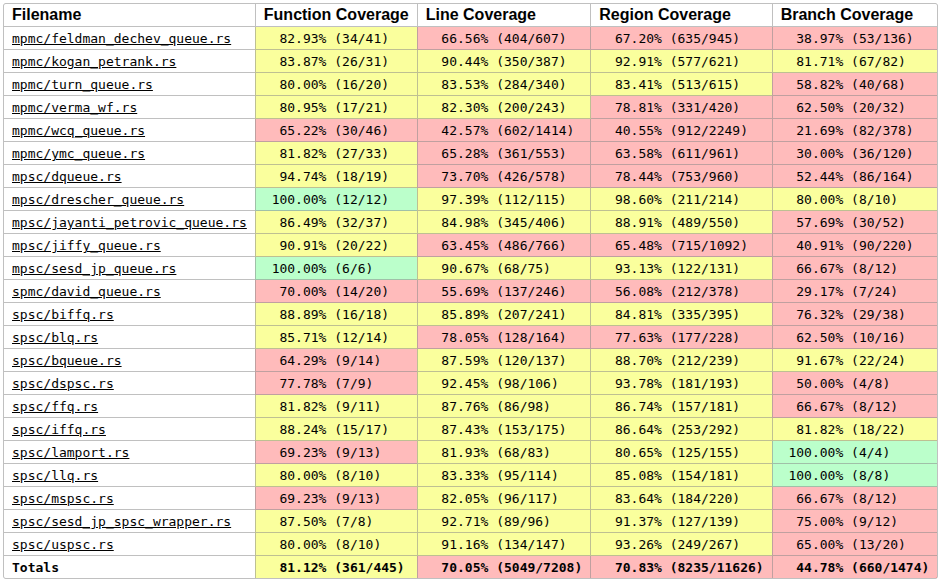
\includegraphics[width=145mm]{images/coverage.png}
    \label{fig:cov}
\end{figure}
